\chapter{Attachments}

\section{Source codes}
\label{sec:source_codes}
\xxx{TODO: add a brief recap of the source codes (maybe not needed)}

\section{GitHub}
\label{sec:github}

The source codes are publicly available on GitHub at \url{https://github.com/cusbg/prankweb}.

The official documentation of the PrankWeb architecture and P2Rank tool is available at \url{https://github.com/cusbg/p2rank-framework/}.

\section{Abbreviations}
\label{sec:abbreviations}
\xxx{TODO: maybe add abbreviations to the end?}

\section{Pocket detail designs}
\label{sec:pocket_detail_designs}

This section contains all pocket detail designs that were considered for displaying more information about a pocket. In the end, the \cref{fig:dialog-4} was chosen. For more information refer to \cref{sec:plugins}.

\begin{figure}
    \centering
    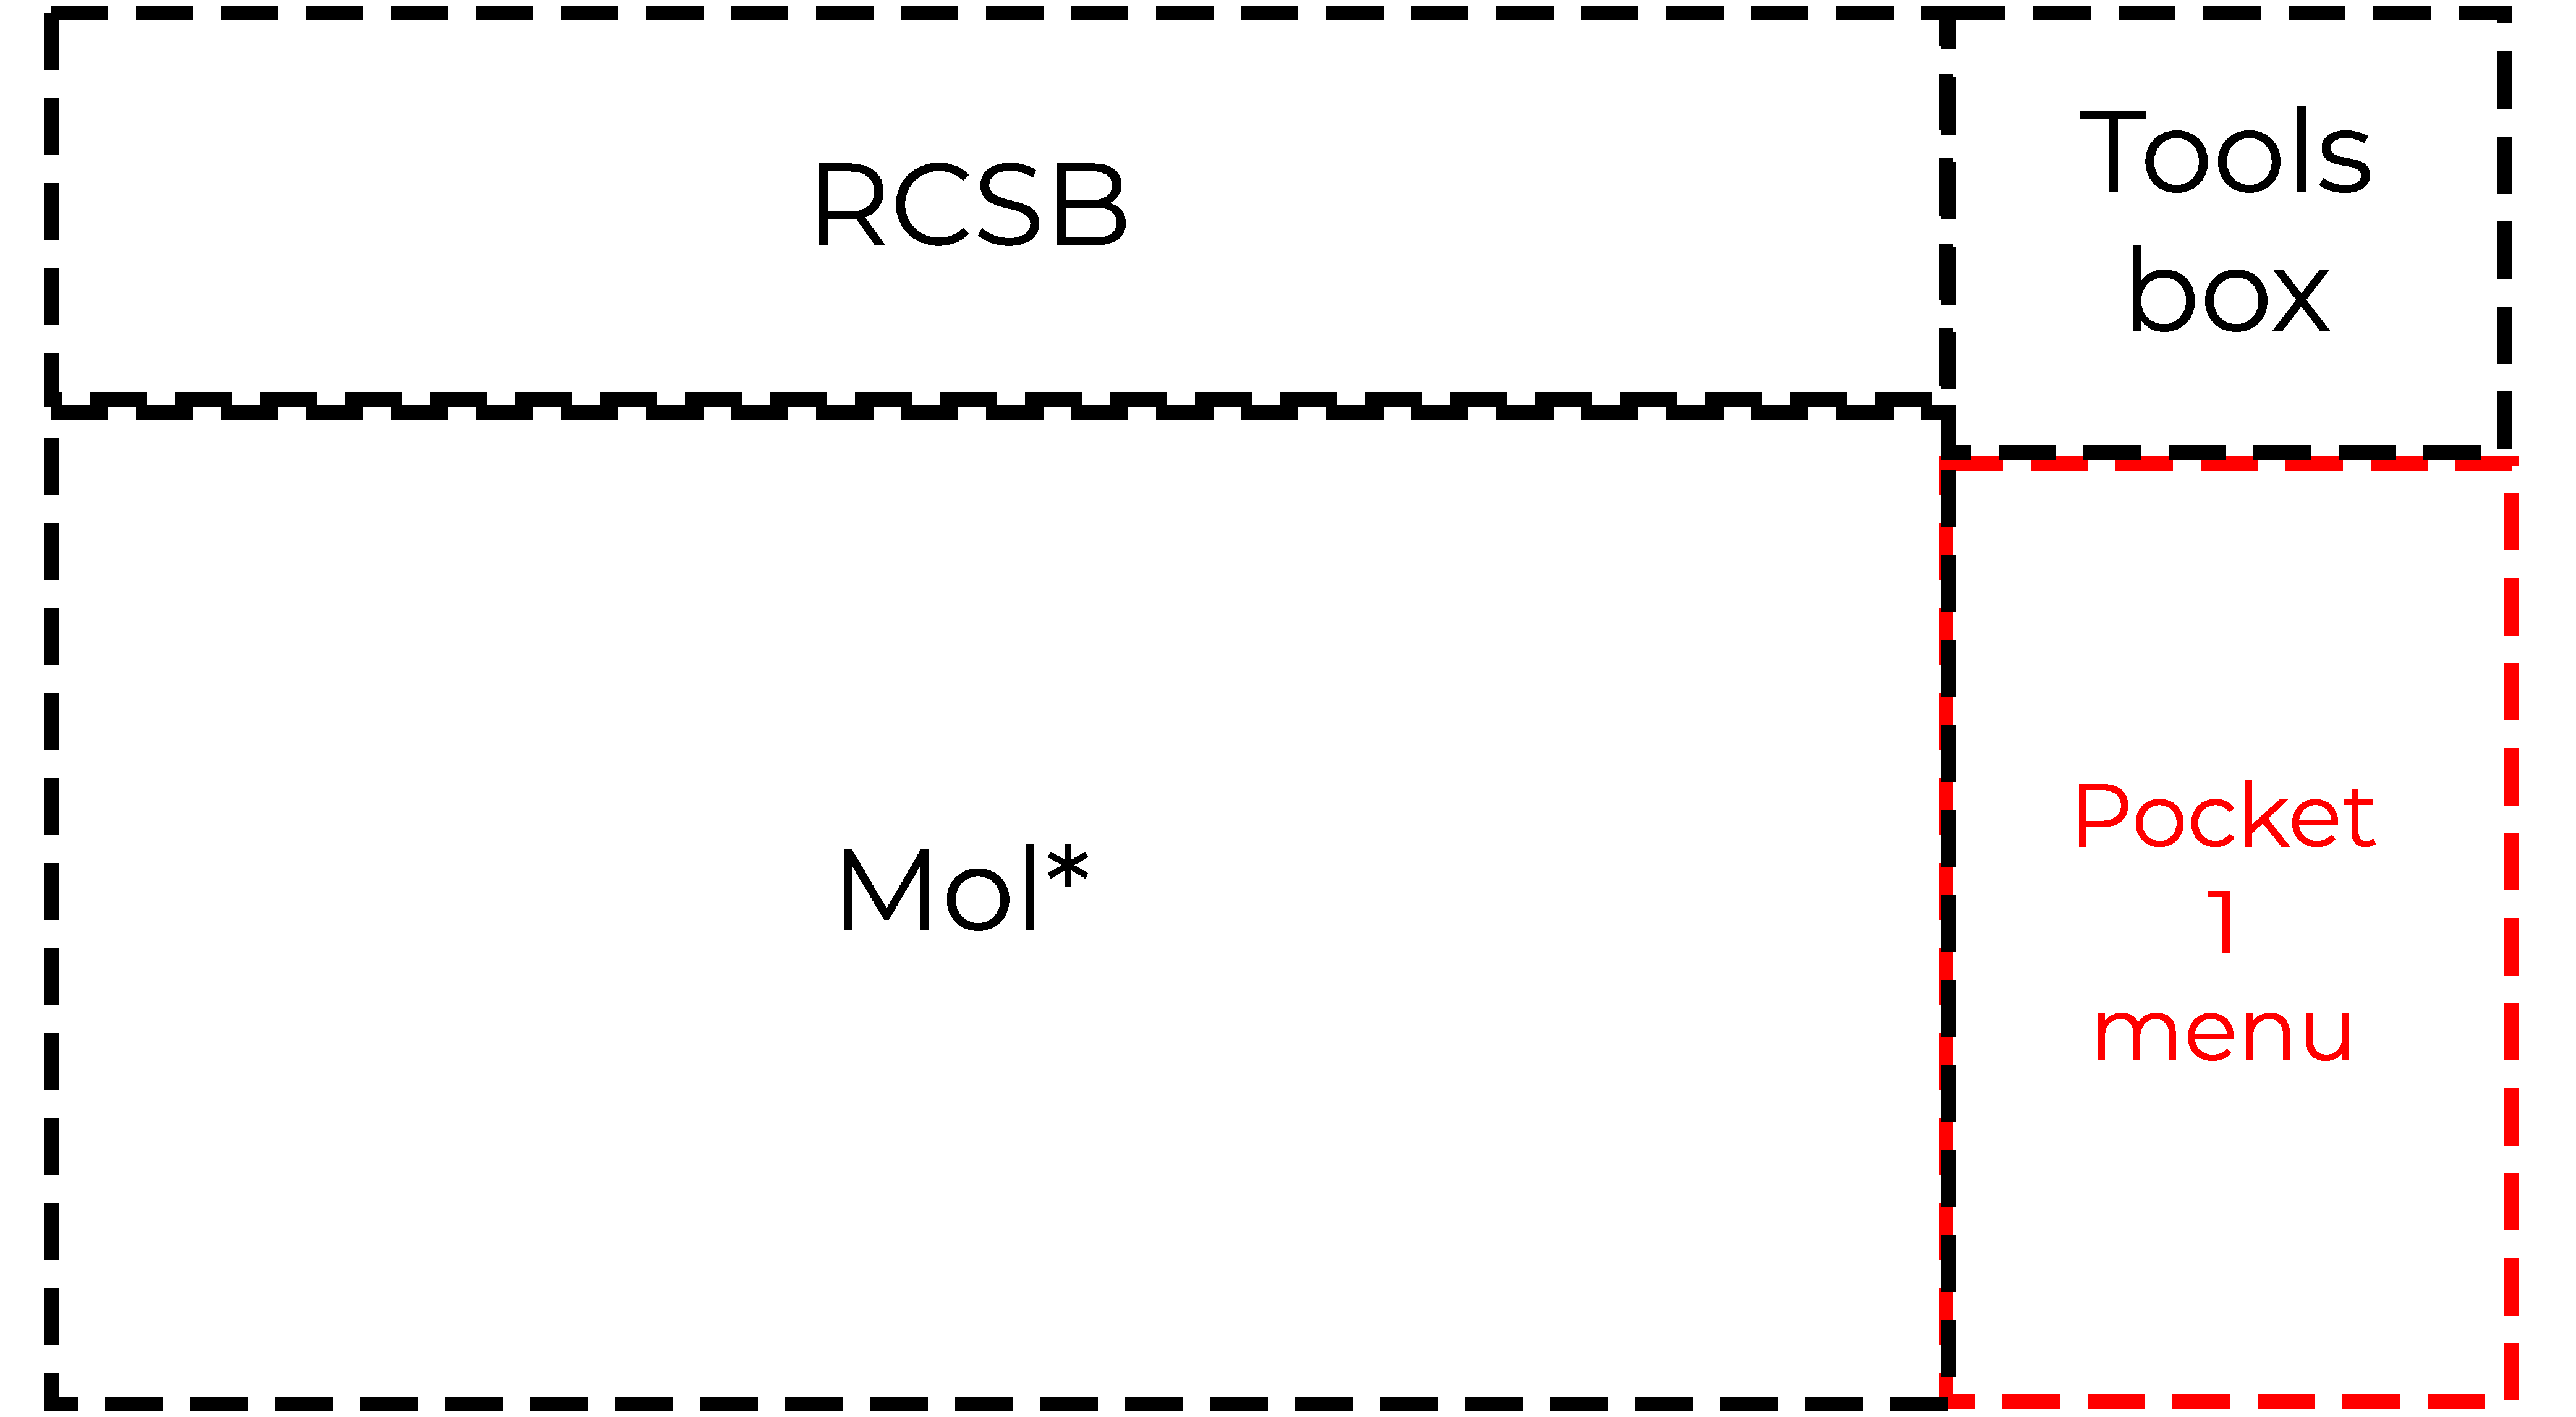
\includegraphics[width=1\linewidth]{img/dialog_1-svg.pdf}
    \caption{The first option for displaying pocket information.}
    \label{fig:figure-1}
\end{figure}

\begin{figure}
    \centering
    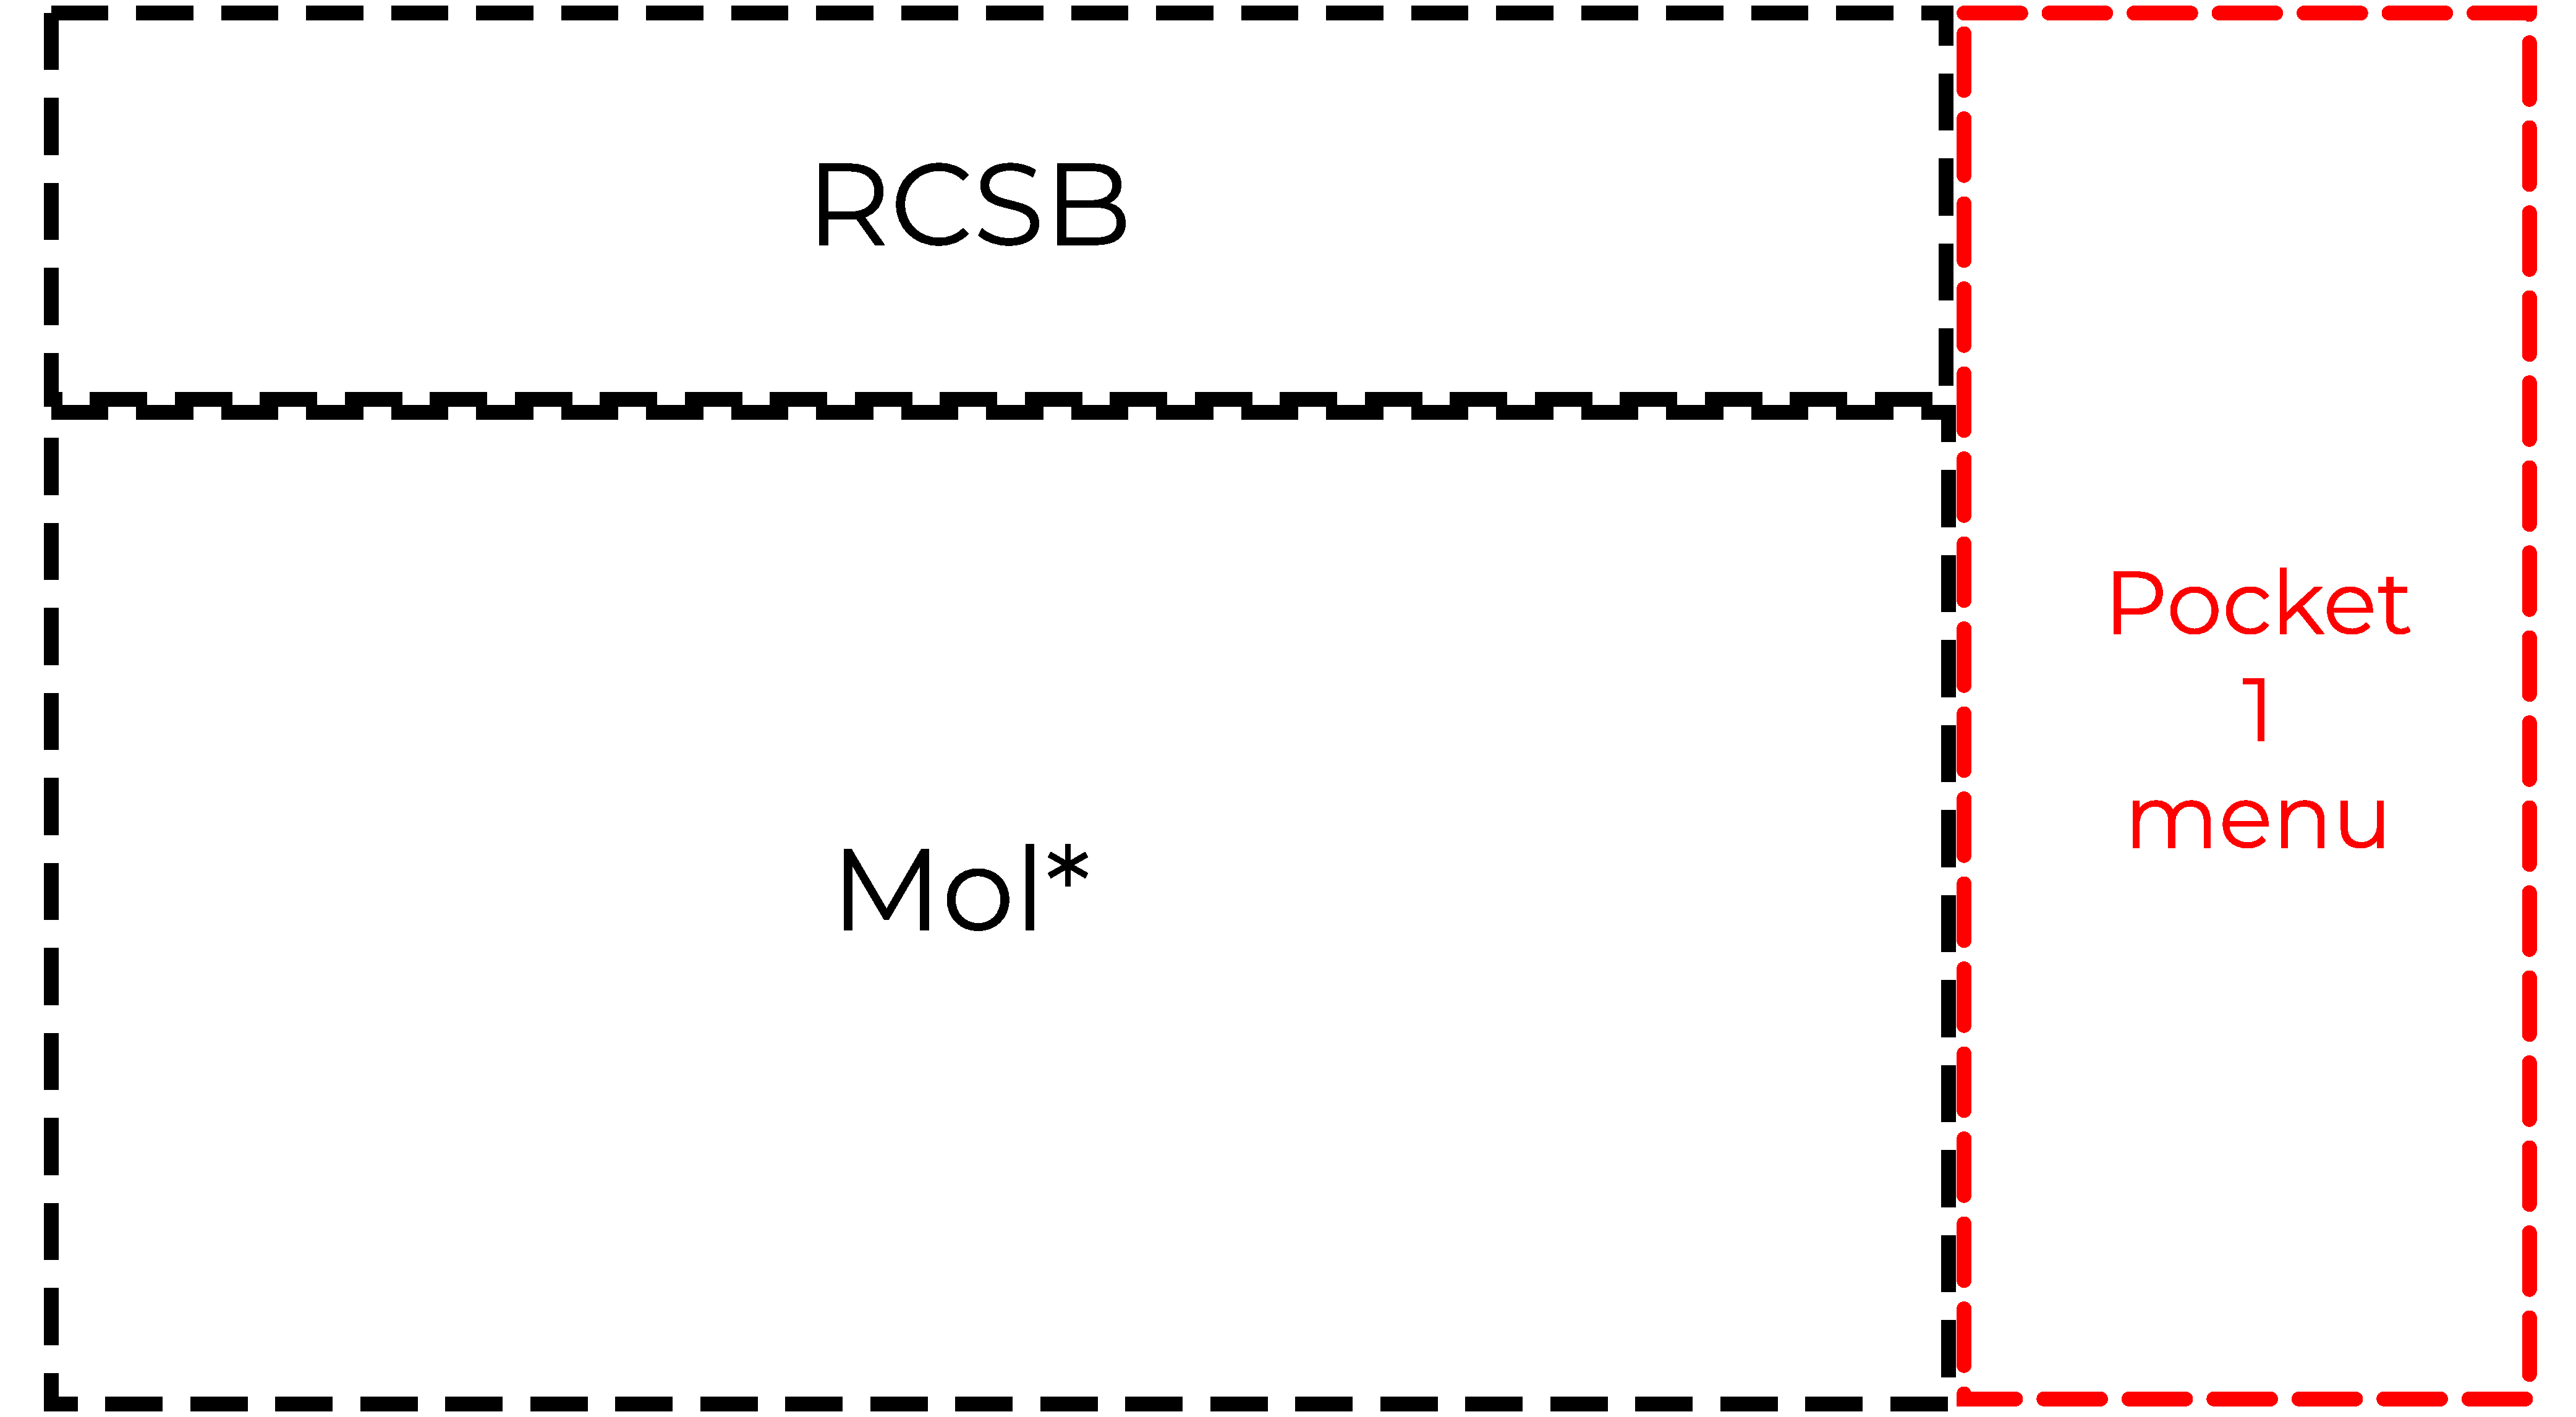
\includegraphics[width=1\linewidth]{img/dialog_2-svg.pdf}
    \caption{The second option for displaying pocket information.}
    \label{fig:figure-2}
\end{figure}

\begin{figure}
	\centering
	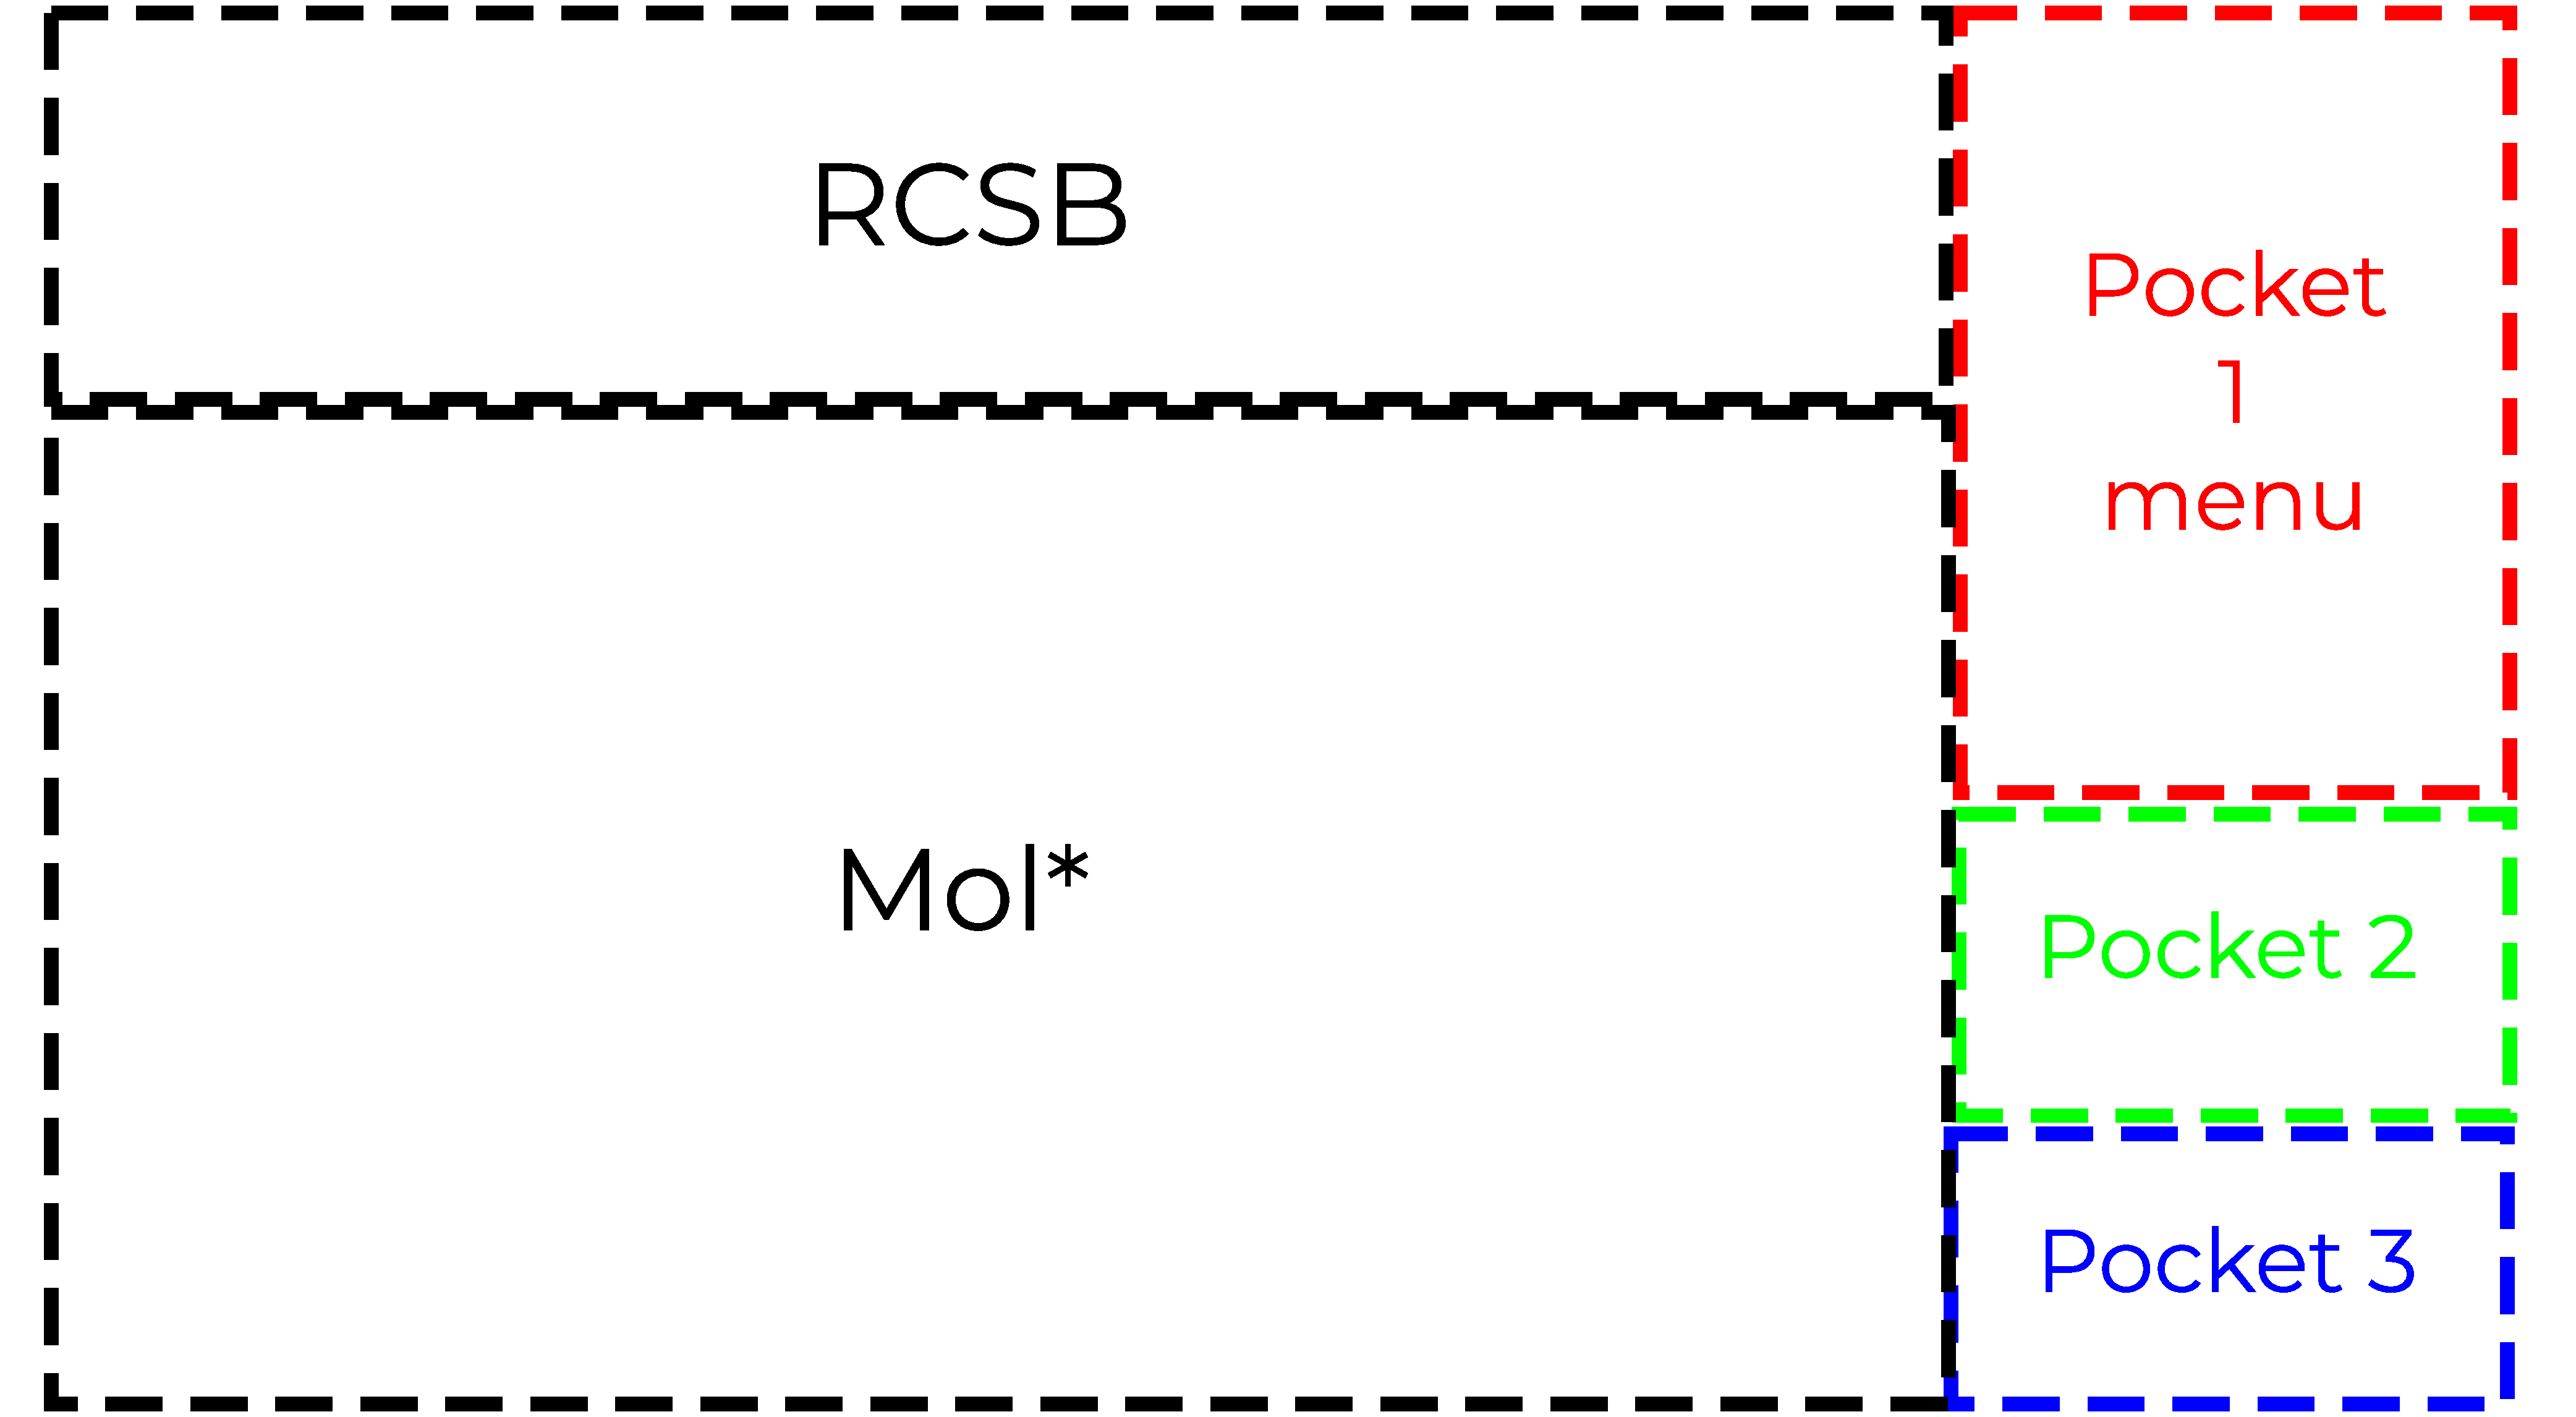
\includegraphics[width=1\linewidth]{img/dialog_3-svg.pdf}
	\caption{The third option for displaying pocket information.}
	\label{fig:figure-3}
\end{figure}

\begin{figure}
	\centering
	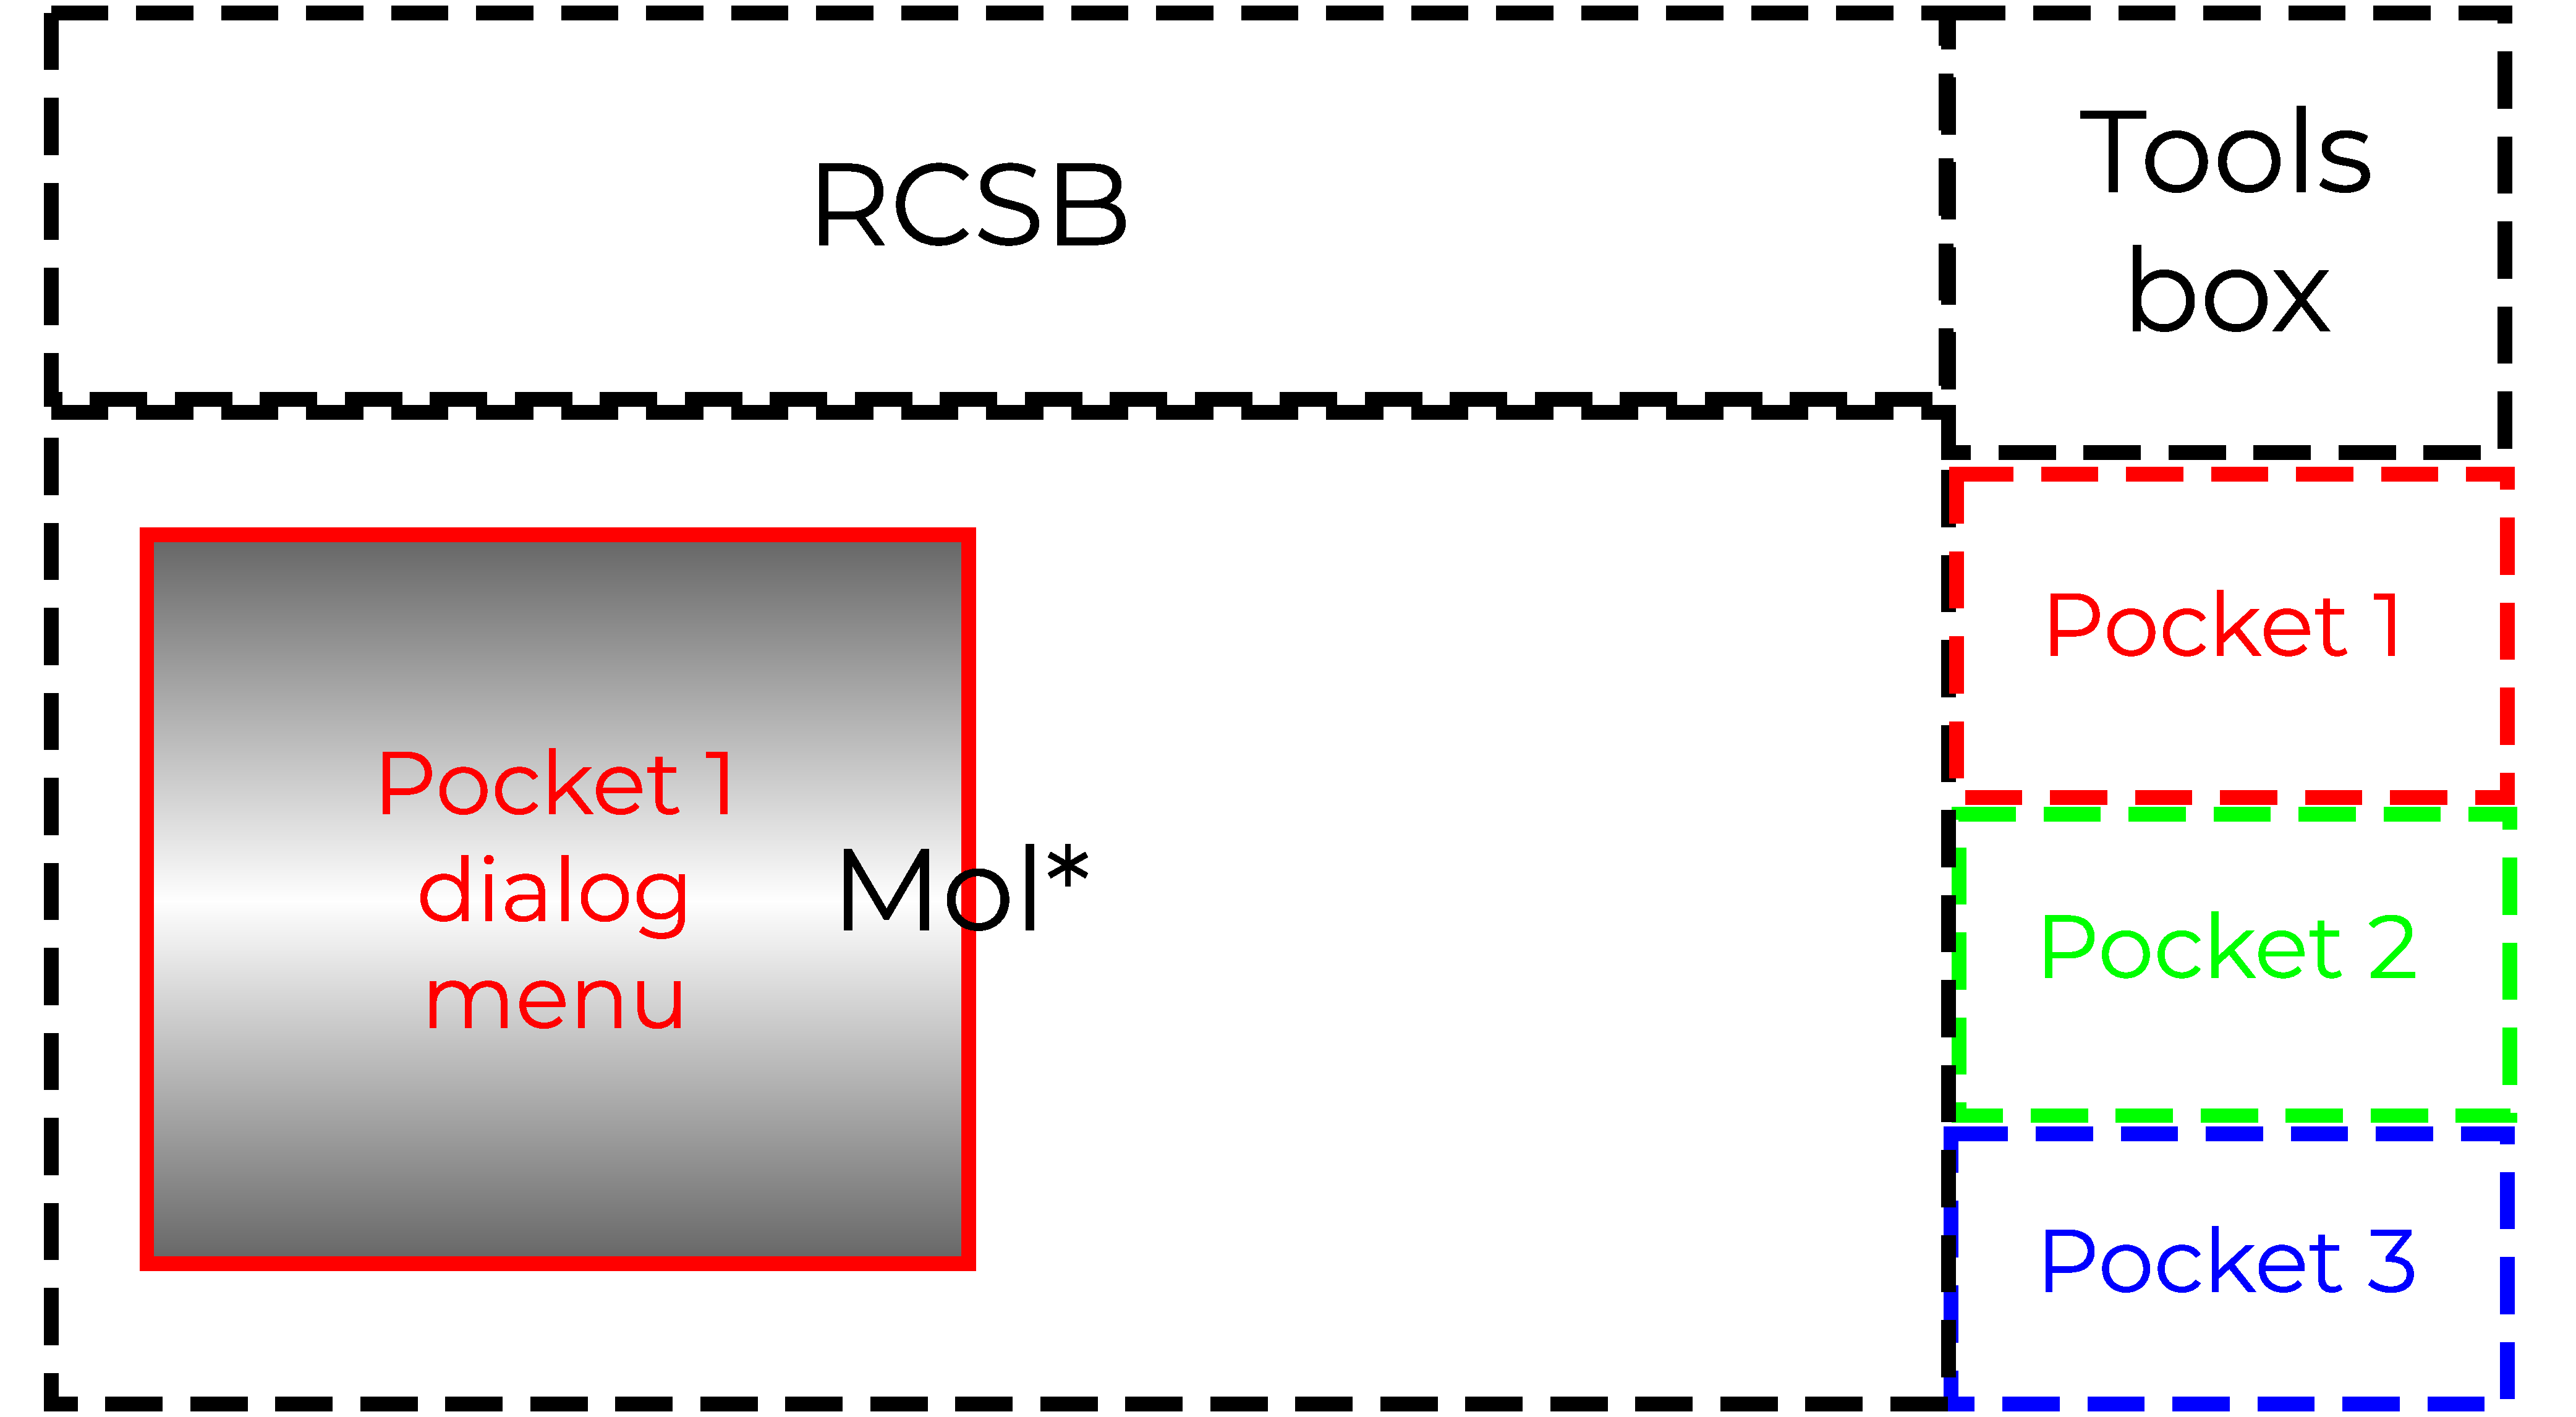
\includegraphics[width=1\linewidth]{img/dialog_4-svg.pdf}
	\caption{The fourth and chosen option for displaying pocket information.}
	\label{fig:dialog-4}
\end{figure}